\documentclass{standalone}

\usepackage{fontspec}
\setmainfont{osifont.ttf}
\fontsize{3.5mm}{4mm}\selectfont

\usepackage{tikz}

\begin{document}
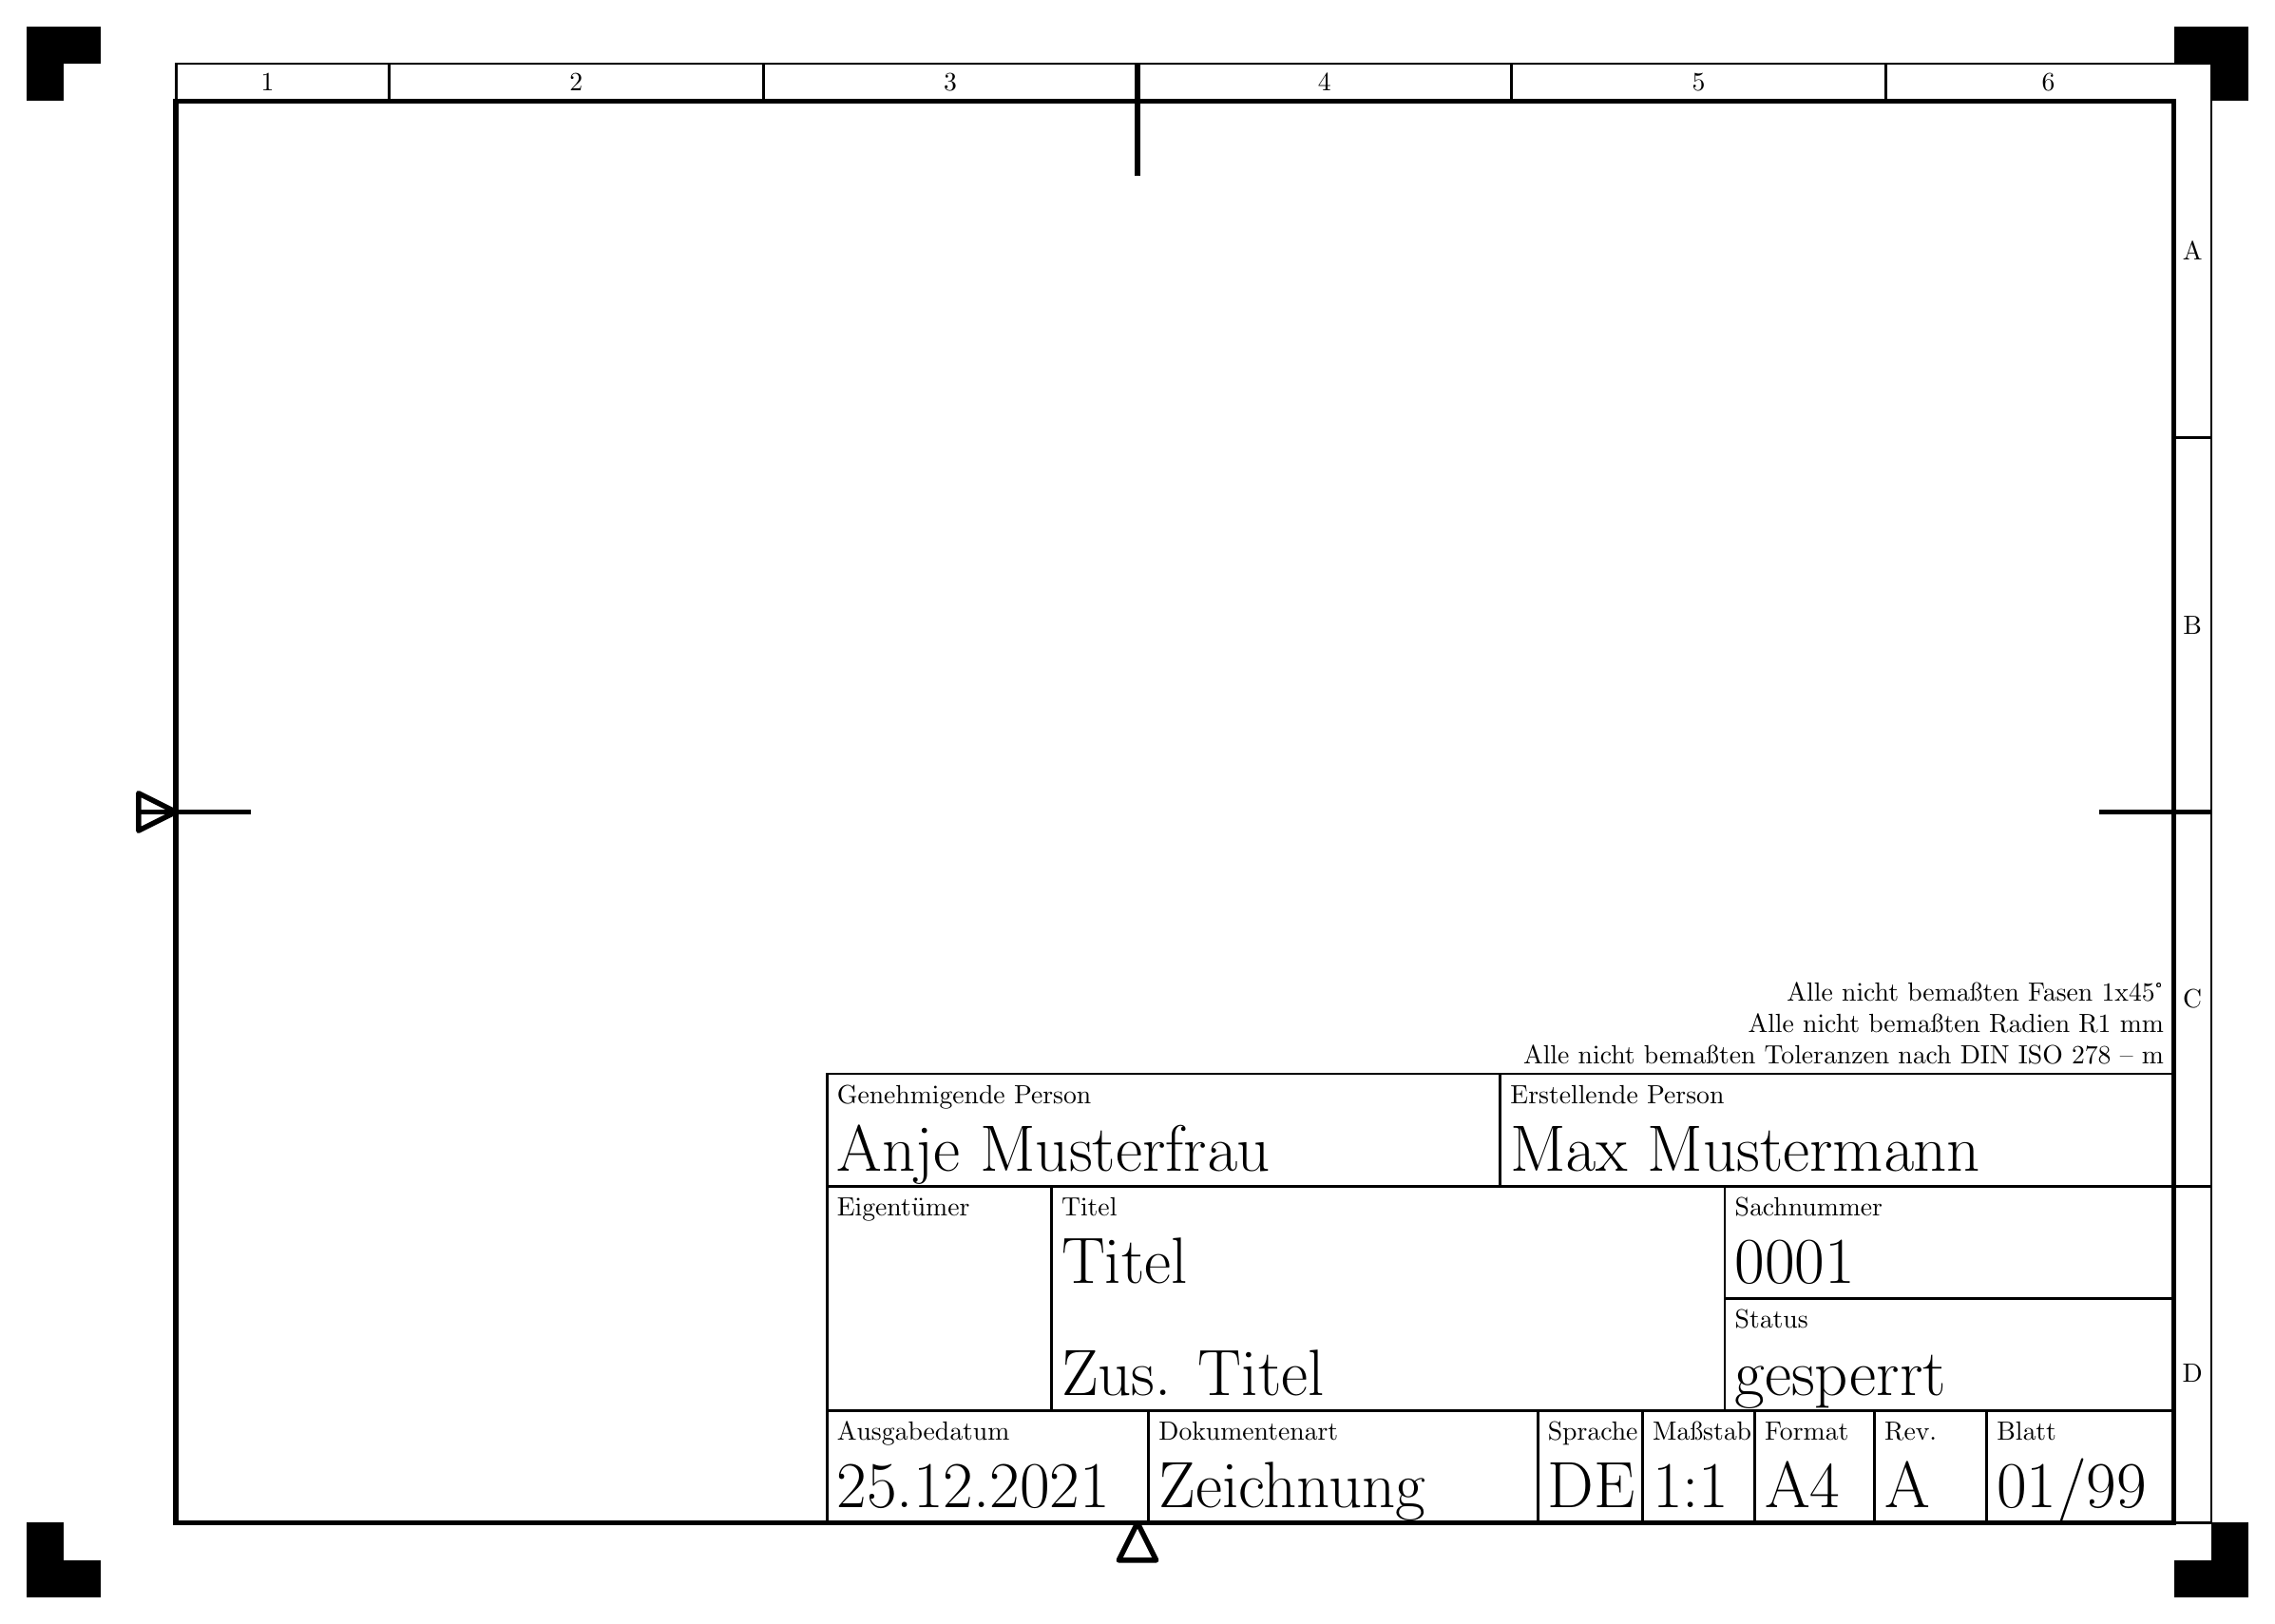
\begin{tikzpicture}[yscale = -1, line width = 0.35mm]
	%\draw[->] (0, 0) -- (0, 1);
	\fill (0, 0) rectangle (10mm, 5mm);
	\fill (0, 0) rectangle (5mm, 10mm);
	\fill (297mm, 0) rectangle (287mm, 5mm);
	\fill (297mm, 0) rectangle (292mm, 10mm);
	\fill (0, 210mm) rectangle (10mm, 205mm);
	\fill (0, 210mm) rectangle (5mm, 200mm);
	\fill (297mm, 210mm) rectangle (287mm, 205mm);
	\fill (297mm, 210mm) rectangle (292mm, 200mm);

	% Zeichenbereich:
	\draw [line width = 0.7mm] (20mm, 10mm) rectangle (287mm, 200mm);

	% Mittellinien:
	\begin{scope}[line width = 0.7mm, line join = round]
		\draw (15mm, 105mm) -- (30mm, 105mm);
		\draw (292mm, 105mm) -- (277mm, 105mm);
		\draw (148.5mm, 5mm) -- (148.5mm, 20mm);
		%\draw (148.5mm, 205mm) -- (148.5mm, 190mm);
		
		% Mittellinien ohne Feldeinteilung:
		\draw (20mm, 105mm) -- (15mm, 102.5mm) -- (15mm, 107.5mm) -- cycle;
		\draw (148.5mm, 200mm) -- (146mm, 205mm) -- (151mm, 205mm) -- cycle;
	\end{scope}

	%Feldeinteilung
	\draw (20mm, 5mm) rectangle (292mm, 200mm);
	\foreach \y in {55mm, 155mm} {
		\draw (287mm, \y) -- (292mm, \y);
	}
	\node at (289.5mm, 30mm) {A};
	\node at (289.5mm, 80mm) {B};
	\node at (289.5mm, 130mm) {C};
	\node at (289.5mm, 180mm) {D};
	
	\foreach \x in {48.5mm, 98.5mm, 198.5mm, 248.5mm} {
		\draw (\x, 5mm) -- (\x, 10mm);
	}
	\node at (32.25mm, 7.5mm) {1};
	\node at (73.5mm, 7.5mm) {2};
	\node at (123.5mm, 7.5mm) {3};
	\node at (173.5mm, 7.5mm) {4};
	\node at (223.5mm, 7.5mm) {5};
	\node at (270.25mm, 7.5mm) {6};

	% Schriftfeld
	\draw (287mm, 200mm) rectangle (107mm, 140mm);

	\begin{scope}[anchor = base west]
		% Zeilen
		\draw (107mm, 155mm) -- (287mm, 155mm);
		\draw (107mm, 185mm) -- (287mm, 185mm);

		% Zeile 1
		\node at (107mm, 144mm) {Genehmigende Person};
		\node at (107mm, 153mm) {\fontsize{10mm}{11mm}\selectfont Anje Musterfrau};
		\node at (197mm, 144mm) {Erstellende Person};
		\node at (197mm, 153mm) {\fontsize{10mm}{11mm}\selectfont Max Mustermann};
		\foreach \x in {197mm} {
			\draw (\x, 140mm) -- (\x, 155mm);
		}

		% Zeile 2
		\node at (107mm, 159mm) {Eigentümer};
		\node at (137mm, 159mm) {Titel};
		\node at (137mm, 168mm) {\fontsize{10mm}{11mm}\selectfont Titel};
		\node at (137mm, 183mm) {\fontsize{10mm}{11mm}\selectfont Zus. Titel};
		\foreach \x in {137mm, 227mm} {
			\draw (\x, 155mm) -- (\x, 185mm);
		}
		\draw (227mm, 170mm) -- (287mm, 170mm);
		\node at (227mm, 159mm) {Sachnummer};
		\node at (227mm, 168mm) {\fontsize{10mm}{11mm}\selectfont 0001};
		\node at (227mm, 174mm) {Status};
		\node at (227mm, 183mm) {\fontsize{10mm}{11mm}\selectfont gesperrt};

		% Zeile 3
		\node at (107mm, 189mm) {Ausgabedatum};
		\node at (107mm, 198mm) {\fontsize{10mm}{11mm}\selectfont 25.12.2021};
		\node at (150mm, 189mm) {Dokumentenart};
		\node at (150mm, 198mm) {\fontsize{10mm}{11mm}\selectfont Zeichnung};
		\node at (202mm, 189mm) {Sprache};
		\node at (202mm, 198mm) {\fontsize{10mm}{11mm}\selectfont DE};
		\node at (216mm, 189mm) {Maßstab};
		\node at (216mm, 198mm) {\fontsize{10mm}{11mm}\selectfont 1:1};
		\node at (231mm, 189mm) {Format};
		\node at (231mm, 198mm) {\fontsize{10mm}{11mm}\selectfont A4};
		\node at (247mm, 189mm) {Rev.};
		\node at (247mm, 198mm) {\fontsize{10mm}{11mm}\selectfont A};
		\node at (262mm, 189mm) {Blatt};
		\node at (262mm, 198mm) {\fontsize{10mm}{11mm}\selectfont 01/99};
		\foreach \x in {150mm, 202mm, 216mm, 231mm, 247mm, 262mm} {
			\draw (\x, 185mm) -- (\x, 200mm);
		}
	\end{scope}

	% Weitere Hinweise
	\begin{scope}[anchor = south east]
		\node [align = right] at (287mm, 140mm) {Alle nicht bemaßten Fasen 1x45°\\Alle nicht bemaßten Radien R1 mm\\Alle nicht bemaßten Toleranzen nach DIN ISO 278 -- m};
	\end{scope}
\end{tikzpicture}
\end{document}
